\documentclass[12pt]{article}

\usepackage{sbc-template}

\usepackage{graphicx,url}

%\usepackage[brazil]{babel}
\usepackage[utf8]{inputenc}
\usepackage{nicefrac}
% Change paragraph identation
\setlength{\parindent}{.8cm}
\usepackage{indentfirst}
\newcommand{\etal}{\textit{et. al}}
\usepackage{float}



\sloppy

\title{Classificação da nota de redação na base de microdados do ENEM 2012 utilizando o algoritmo \emph{k-Nearest Neighbors}}

\author{Jonathan Coutinho Luz de Queiroz\inst{1} \\ Guilherme Lima Bernal\inst{1}}
\address{Instituto de Matemática -- Universidade Federal da Bahia (UFBA)
\email{jonathanqueiroz@dcc.ufba.br}
}

\newcommand{\reffig}[1]{Fig.~\ref{fig:#1}}
\newcommand{\reftab}[1]{Tabela~\ref{tab:#1}}

\geometry{lmargin=2.2cm, rmargin=2.2cm, tmargin=2.2cm, bmargin=2.2cm}
\setlength\tabcolsep{4pt}
\begin{document}

\maketitle

\begin{resumo}
Neste trabalho, tomamos como base o algoritmo k-Nearest Neighbors (k-NN) para a predição da nota de redação na base de microdados do ENEM 2012.
O primeiro passo consistiu na realização de uma análise estatística sobre a base de dados.
Em seguida, preparamos a base para a aplicação do algoritmo de classificação.
Depois disso, amparados na análise estatística previamente realizada, desenvolvemos uma versão inicial do algoritmo de classificação.
Finalmente, refinamos o algoritmo desenvolvido através de experimentos e analisamos a sua acurácia.
\end{resumo}

\section{Introdução}
\label{sec:intro}
O principal objetivo deste trabalho consistiu no desenvolvimento de um algoritmo de classificação da nota de redação de candidatos do ENEM.
Para isso, utilizamos a base de micro-dados do ENEM 2012, cujos registros correspondem a candidatos e cujos atributos incluem nome, idade, sexo, localização, tipo de escola, notas nas provas objetivas, nota na prova de redação, dentre outros.
Mais precisamente, consideramos um subconjunto da base composto por 50.000 candidatos, dos quais 14.672 foram descartados de imediato por não terem feito a prova de redação.

O primeiro passo do trabalho consistiu na realização de uma análise estatística sobre a base de dados, a qual permitiu a identificação dos atributos mais correlacionados à nota de redação.
Em seguida, a base de dados foi pré-processada para viabilizar a aplicação do algoritmo de classificação.
Finalmente, um algoritmo de classificação foi desenvolvido e iterativamente refinado através de experimentos.

O restante deste artigo está organizado da seguinte maneira.
A seção~\ref{sec:analise-estatistica} sumariza a análise estatística, apresentando os resultados mais relevantes para a classificação das notas.
A seção~\ref{sec:pre-processamento} descreve o processo de preparação da base de dados para utilização no algoritmo de classificação.
A seção~\ref{sec:classificacao} descreve o algoritmo genérico de classificação e então detalha a sua aplicação na base de dados do ENEM, avaliando também os resultados obtidos.
Finalmente, a seção~\ref{sec:conclusao} conclui o trabalho e sugere possíveis direções a serem tomadas em trabalhos futuros.

\section{Análise estatística}
\label{sec:analise-estatistica}
O primeiro passo da análise estatística consistiu no estudo isolado dos principais atributos da base (idade, sexo, região, localização, tipo de escola e nota de redação).
%Em seguida, foi feita uma comparação entre as idades e as notas de redação dos candidatos de cada região do país.
%Finalmente, analisamos a correlação entre a nota de redação e diversos outros atributos (idade, sexo, tipo de escola, localização, ano de conclusão do Ensino Médio, notas nas demais provas, deficiência mental e deficiência física).
Em seguida, analisamos a correlação entre a nota de redação e diversos outros atributos (idade, sexo, tipo de escola, tipo de localização, ano de conclusão do Ensino Médio, notas nas demais provas, deficiência mental e deficiência física).

Removemos dois \emph{outliers} de acordo com a idade: um candidato de 7 anos e outro de 114 anos.
Após a remoção desses dois candidatos, a idade passou a variar entre 12 e 70 anos (inclusive), o que indica que os dois registros removidos estão incorretos.
Ainda que não estejam, no entanto, a remoção de dois registros dentre mais de 30.000 é estatisticamente insignificamente e é justificada pela melhoria que isso proporciona na visualização dos gráficos.\footnote{Antes da remoção desses dois registros, mais de $\nicefrac{1}{3}$ da área do histograma de idades era ocupado por valores de 70 a 114, mesmo havendo apenas um registro com valor nessa faixa.}
%Restaram 35.326 candidatos.
% TODO: move to introduction?

% \subsection{Estatísticas gerais da base}
% \label{subsec:estatisticas-gerais}
% %Antes de iniciarmos uma análise mais aprofundada da base de dados, coletamos algumas estatísticas a respeito dos seus principais atributos, dispostas nos gráficos a seguir.
% Coletamos algumas estatísticas a respeito dos principais atributos da base, dispostas nos gráficos a seguir.
% Conforme evidenciado pela \reffig{candidatos-por-idade}, a maioria dos candidatos possui até 20 anos de idade.
% Mais precisamente, dentre os 35.326 candidatos da base, 21.616 (61.2\%) possuem até 20 anos de idade e 28.205 (79.84\%) possuem até 25 anos de idade.
% Além disso, como mostra \reffig{candidatos-por-sexo}, há mais candidatos do sexo feminino (59.0\%) do que candidatos do sexo masculino (41.0\%).

% \begin{minipage}{.5\textwidth}
%     \begin{figure}[H]
%     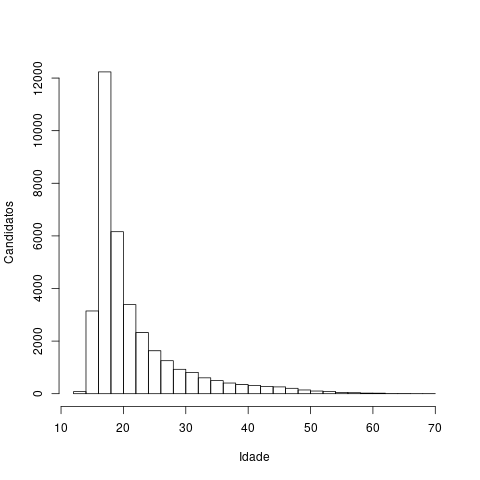
\includegraphics[width=.9\linewidth]{../geral_candidatos-por-idade.png}
%     \caption{Candidatos por idade.}
%     \label{fig:candidatos-por-idade}
%     \end{figure}
% \end{minipage}%
% \begin{minipage}{.5\textwidth}
%     \begin{figure}[H]
%     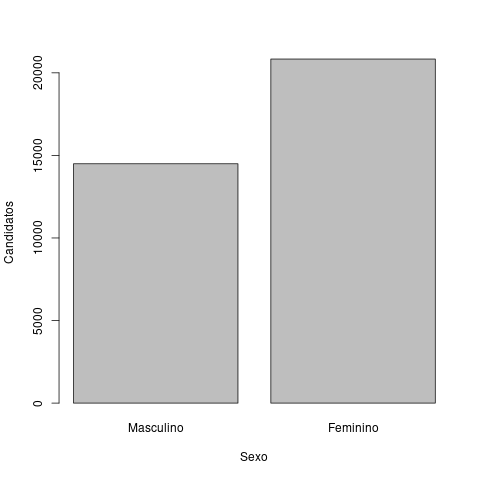
\includegraphics[width=.9\linewidth]{../geral_candidatos-por-sexo.png}
%     \caption{Candidatos por sexo.}
%     \label{fig:candidatos-por-sexo}
%     \end{figure}
% \end{minipage}


% \vspace{1cm}
% Conforme evidenciado pela \reffig{candidatos-por-regiao}, a maioria dos candidatos (68.4\%) está concentrada nas regiões Nordeste e Sudeste.
% Além disso, de acordo com a \reffig{candidatos-por-localizacao}, a maioria dos candidatos não informou a localização (zona urbana ou zona rural).
% Dentre aqueles que informaram, no entanto, a enorme maioria vive na zona urbana.
% \begin{minipage}{.5\textwidth}
%     \begin{figure}[H]
%     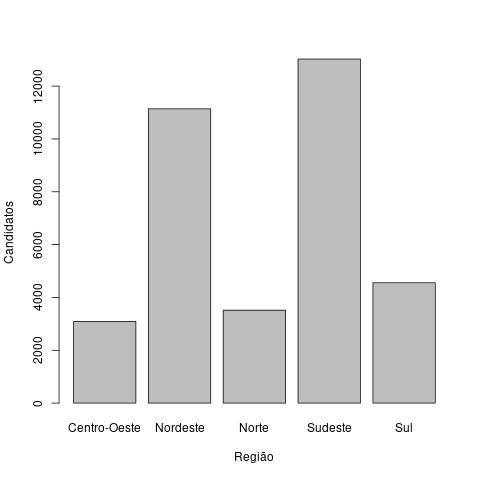
\includegraphics[width=.9\linewidth]{../geral_candidatos-por-regiao.png}
%     \caption{Candidatos por região.}
%     \label{fig:candidatos-por-regiao}
%     \end{figure}
% \end{minipage}%
% \begin{minipage}{.5\textwidth}
%     \begin{figure}[H]
%     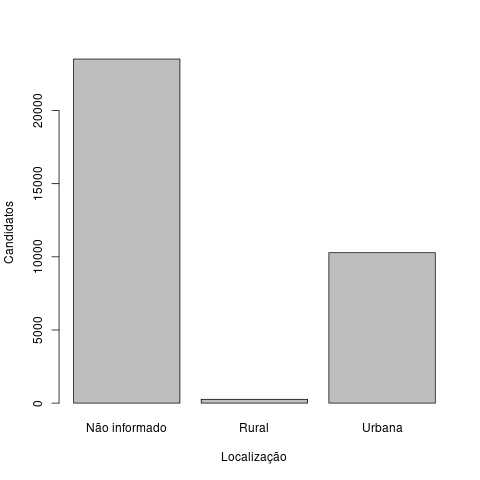
\includegraphics[width=.9\linewidth]{../geral_candidatos-por-localizacao.png}
%     \caption{Candidatos por localização.}
%     \label{fig:candidatos-por-localizacao}
%     \end{figure}
% \end{minipage}


% \vspace{1cm}
% De acordo com a \reffig{candidatos-por-escola}, a maioria dos candidatos não informou o tipo de escola que frequentou.
% Dentre aqueles que informaram, no entanto, a grande maioria estudou em escola pública.
% A \reffig{candidatos-por-nota} evidencia a concentração das notas de redação em torno da mediana.
% Dos 35.326 canditados, apenas 1507 (4.27\%) obtiveram nota abaixo de 200 e apenas 1.174 (3.32\%) obtiveram nota acima de 800.

% \begin{minipage}{.5\textwidth}
%     \begin{figure}[H]
%     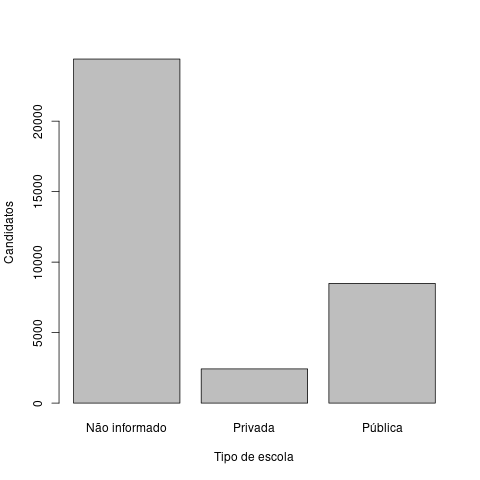
\includegraphics[width=\linewidth]{../geral_candidatos-por-escola.png}
%     \caption{Candidatos por tipo de escola.}
%     \label{fig:candidatos-por-escola}
%     \end{figure}
% \end{minipage}%
% \begin{minipage}{.5\textwidth}
% \begin{figure}[H]
% \centering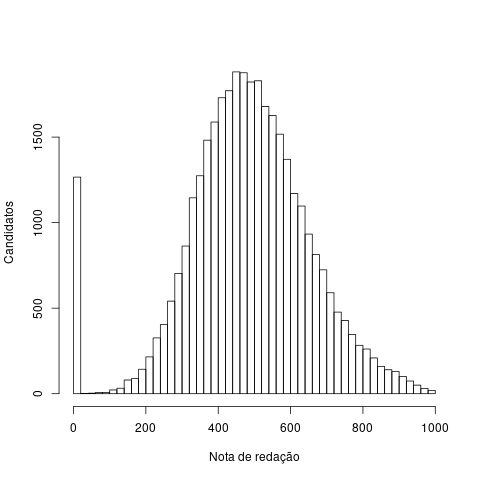
\includegraphics[width=\linewidth]{../geral_candidatos-por-nota.png}
% \caption{Candidatos por nota de redação.}
% \label{fig:candidatos-por-nota}
% \end{figure}
% \end{minipage}

% \iffalse
% \subsection{Estatísticas por região}
% O próximo passo consistiu em gerar estatísticas separadas para cada região, visando a identificação de possíveis associações entre a região do candidado e demais atributos.
% Os resultados são apresentados a seguir.

% \subsubsection{Idade}
% Conforme evidenciado pela \reftab{idade-por-regiao} e pela \reffig{idade-por-regiao}, a correlação entre a região do candidato e a idade é, em geral, desprezível. Essa correlação se acentua um pouco no caso da região Norte, cujos candidatos tendem a ser, em média, aproximadamente um ano mais velhos, mas ainda assim é pouco significativa.

% \begin{minipage}{.5\textwidth}
%     \begin{table}[H]
%     \begin{tabular}{ c c c c c }
%       \textbf{Região}  & \textbf{Candidatos} & \textbf{Média} & \textbf{Mediana} & \textbf{Desvio-padrão} \\
%       Brasil           & 35.326              & 22.03          & 19               & 7.48 \\
%       Norte            & 3.517               & 22.94          & 20               & 7.52 \\
%       Nordeste         & 11.140              & 22.03          & 19               & 7.15 \\
%       Sudeste          & 13.024              & 21.69          & 19               & 7.55 \\
%       Sul              & 4.555               & 22.01          & 19               & 7.76 \\
%       Centro-Oeste     & 3.090               & 22.41          & 19               & 7.81 \\
%     \end{tabular}
%     \caption{Idade dos candidatos por região.}
%     \label{tab:idade-por-regiao}
%     \end{table}
% \end{minipage}%
% \begin{minipage}{.5\textwidth}
%     \begin{figure}[H]
%     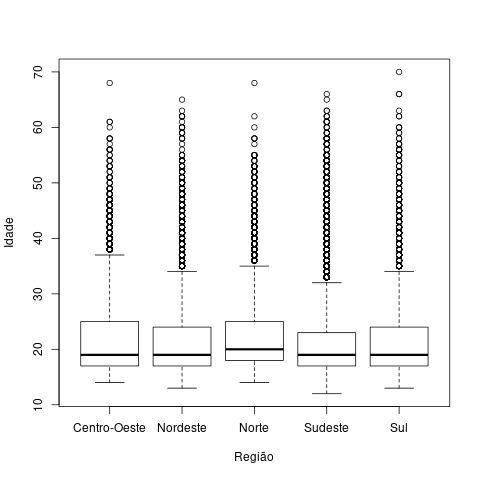
\includegraphics[width=\linewidth]{../regiao_idade.png}
%     \caption{Idade dos candidatos por região.}
%     \label{fig:idade-por-regiao}
%     \end{figure}
% \end{minipage}

% \subsubsection{Nota da redação}
% A \reftab{nota-por-regiao} e a \reffig{nota-por-regiao} revelam uma leve associação entre a região do candidato e a nota da redação. Mais especificamente, candidatos do Sudesde, e em seguida do Sul, tendem a apresentar notas mais altas que os candidatos das demais regiões. A região com pior desempenho foi a Norte.

% \begin{minipage}{.5\textwidth}
%     \begin{table}[H]
%     \begin{tabular}{ c c c c c }
%       \textbf{Região}  & \textbf{Candidatos} & \textbf{Média} & \textbf{Mediana} & \textbf{Desvio-padrão} \\
%       Brasil           & 35.326              & 491.49          & 500             & 173.84 \\
%       Norte            & 3.517               & 469.24          & 460             & 174.00 \\
%       Nordeste         & 11.140              & 478.70          & 480             & 176.39 \\
%       Sudeste          & 13.024              & 513.09          & 520             & 172.16 \\
%       Sul              & 4.555               & 489.52          & 500             & 169.68 \\
%       Centro-Oeste     & 3.090               & 474.77          & 480             & 167.78 \\
%     \end{tabular}
%     \caption{Nota de redação dos candidatos por região.}
%     \label{tab:nota-por-regiao}
%     \end{table}
% \end{minipage}%
% \begin{minipage}{.5\textwidth}
%     \begin{figure}[H]
%     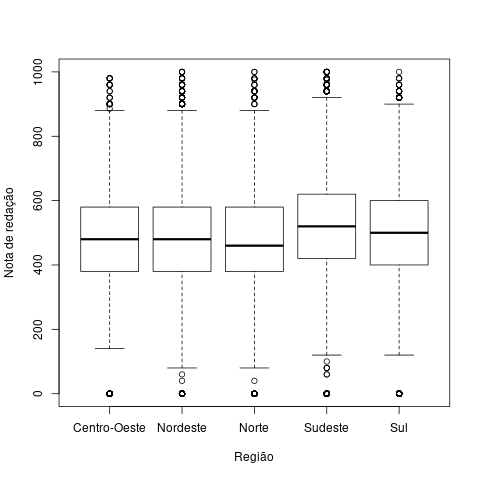
\includegraphics[width=\linewidth]{../regiao_nota.png}
%     \caption{Nota de redação dos candidatos por região.}
%     \label{fig:nota-por-regiao}
%     \end{figure}
% \end{minipage}
% \fi

\subsection{Análise de correlações}
Elegemos alguns atributos para avaliar a existência de possíveis correlações com as notas de redação, a saber: idade, sexo, tipo de escola (pública ou privada), localização (zona urbana ou zona rural), ano de conclusão do Ensino Médio e notas nas provas objetivas.
Dentre todos esses atributos, aqueles que apresentaram maior correlação com a nota de redação foram as notas nas provas objetivas.

% \subsubsection{Idade}
% %TODO: melhorar essa imagem
% A \reffig{correlacao-idade} apresenta as notas de redação em função da idade dos candidatos e aponta para a inexistência de correlação significativa entre esses dois atributos.
% De fato, o coeficiente de correlação de Pearson entre essas duas variáveis vale aproximadamente $-0.11$, o que confirma essa hipótese.

% \begin{figure}[H]
% \centering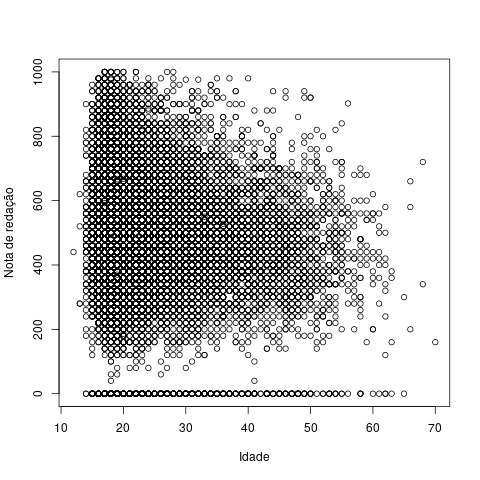
\includegraphics[width=.5\linewidth]{../correlacao_idade.png}
% \caption{Notas de redação em função da idade.}
% \label{fig:correlacao-idade}
% \end{figure}

% \subsubsection{Sexo}
% A \reffig{correlacao-sexo} indica que a diferença de desempenho entre candidatos do sexo masculino e do sexo feminino é pequena.

% \begin{figure}[H]
% \centering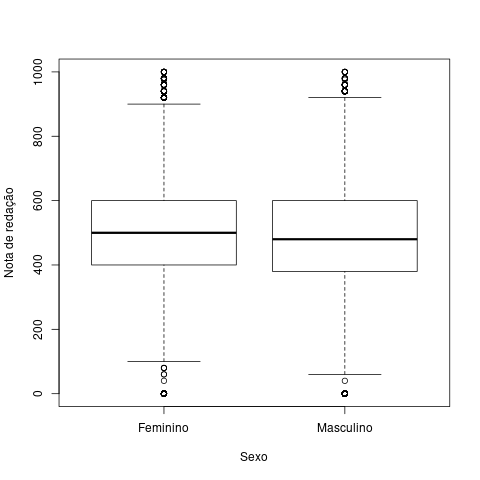
\includegraphics[width=.5\linewidth]{../correlacao_sexo.png}
% \caption{Distribuição das notas de redação para candidatos de cada sexo.}
% \label{fig:correlacao-sexo}
% \end{figure}

% \subsubsection{Tipo de escola}
% A \reffig{correlacao-escola} evidencia uma associação entre a nota da redação e o tipo da escola na qual o candidato estudou.
% Mais especificamente, estudantes de escolas particulares tendem a obter notas mais altas.
% %TODO: ineflizmente, naoad pra usar iso na predicao porque...

% \begin{figure}[H]
% \centering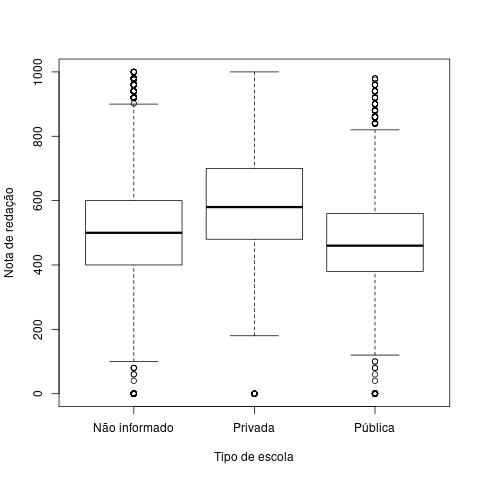
\includegraphics[width=.5\linewidth]{../correlacao_escola.png}
% \caption{Distribuição das notas de redação para estudantes de escolas públicas e de escolas privadas.}
% \label{fig:correlacao-escola}
% \end{figure}

% \subsubsection{Localização}
% A \reffig{correlacao-localizacao} evidencia uma associação entre a nota da redação e a localização do candidato (zona urbana ou zona rural).
% Mais especificamente, candidatos da zona urbana tendem a obter notas mais altas.
% Na subseção~\ref{subsec:estatisticas-gerais}, mostramos que, dentre os candidatos que informaram a localização, a enorme maioria vive na zona urbana.
% A semelhança, na \reffig{correlacao-localizacao}, entre os gráficos dos candidatos que vivem na zona urbana e dos candidatos que não informaram a localização é um possível indício de que a maioria dos candidatos que não informaram localização também vive na zona urbana.

% \begin{figure}[H]
% \centering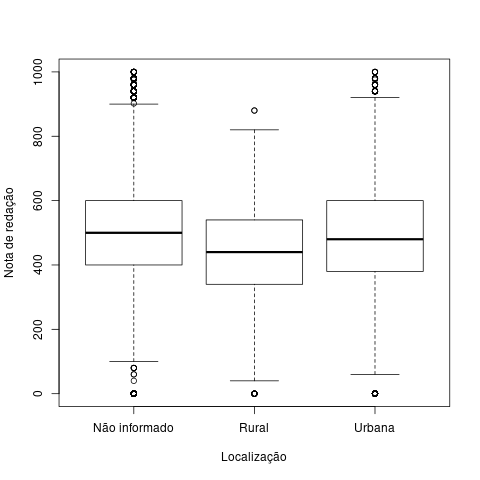
\includegraphics[width=.44\linewidth]{../correlacao_localizacao.png}
% \caption{Distribuição das notas de redação para estudantes da zona urbana e da zona rural.}
% \label{fig:correlacao-localizacao}
% \end{figure}

% \subsubsection{Ano de conclusão do Ensino Médio}
% A \reffig{correlacao-ano-concluiu} aponta para a inexistência de correlação significativa entre a nota da redação e o ano no qual o candidato concluiu o Ensino Médio.\footnote{O valor ``.'' indica que o ano de conclusão do Ensino Médio não foi informado.}
% \begin{figure}[H]
% \centering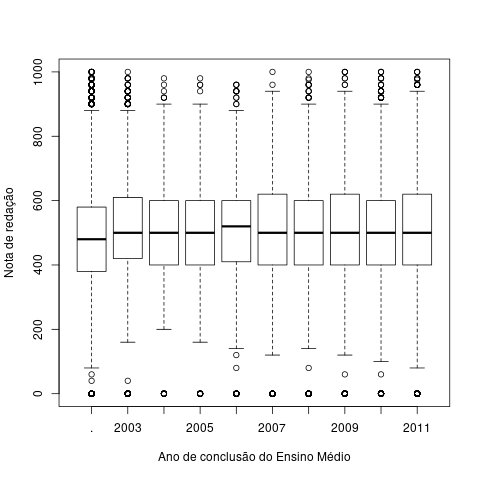
\includegraphics[width=.44\linewidth]{../correlacao_ano_concluiu.png}
% \caption{Distribuição das notas de redação em função do ano de conclusão do Ensino Médio.}
% \label{fig:correlacao-ano-concluiu}
% \end{figure}

% \subsubsection{Notas nas demais provas}
As Figuras~\ref{fig:correlacao-nota-ch}--\ref{fig:correlacao-nota-mt} apresentam uma evidência da existência de correlação positiva entre as notas obtidas pelos candidatos em redação e nas demais provas.
De fato, os coeficientes de correlação de Pearson apresentados na \reftab{coeficiente-pearson-por-prova} confirmam essa hipótese.
Ainda de acordo com a \reftab{coeficiente-pearson-por-prova}, a maior correlação ocorre com as provas de Ciências Humanas e Linguagens e Códigos.
%TODO: footnote dizendo que foram desconsiderados candidatos que faltaram

\vspace{-0.8cm}
\begin{minipage}{.5\textwidth}
    \begin{figure}[H]
    \centering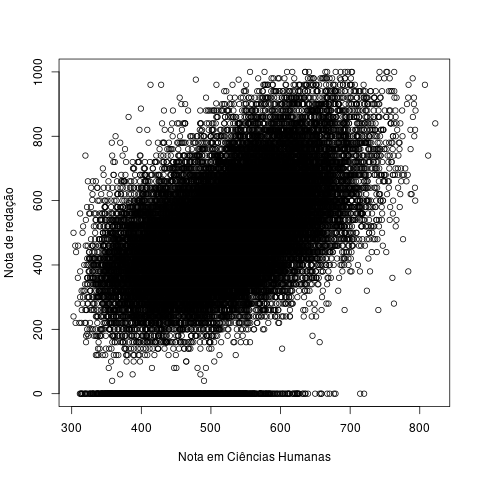
\includegraphics[width=.86\linewidth]{../correlacao_nota_ch.png}
    \caption{Notas de redação em função das notas em Ciências Humanas.}
    \label{fig:correlacao-nota-ch}
    \end{figure}
\end{minipage}%
\begin{minipage}{.5\textwidth}
    \begin{figure}[H]
    \centering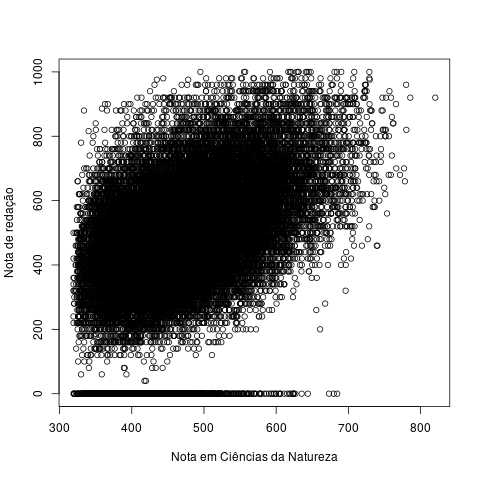
\includegraphics[width=.86\linewidth]{../correlacao_nota_cn.png}
    \caption{Notas de redação em função das notas em Ciências da Natureza.}
    \label{fig:correlacao-nota-cn}
    \end{figure}
\end{minipage}

\begin{minipage}{.5\textwidth}
    \begin{figure}[H]
    \centering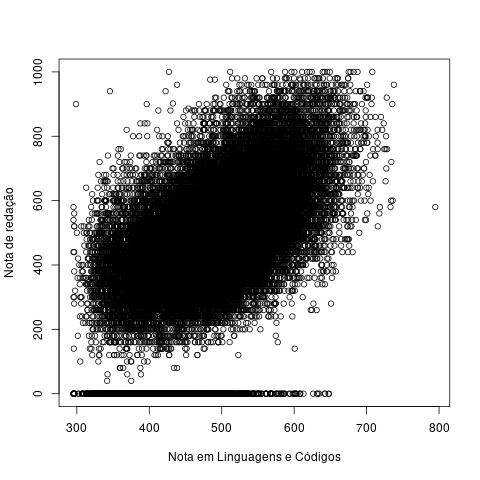
\includegraphics[width=.86\linewidth]{../correlacao_nota_lc.png}
    \caption{Notas de redação em função das notas em Linguagens e Códigos.}
    \label{fig:correlacao-nota-lc}
    \end{figure}
\end{minipage}%
\begin{minipage}{.5\textwidth}
    \begin{figure}[H]
    \centering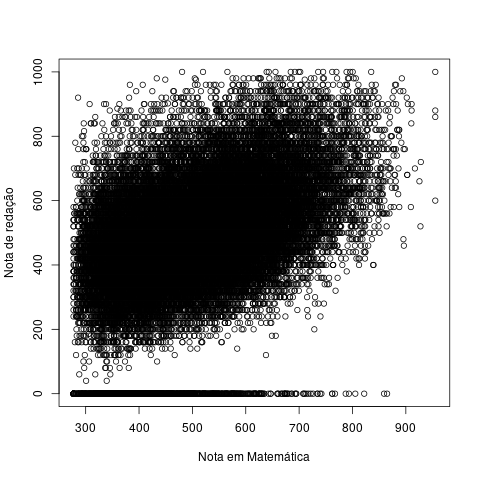
\includegraphics[width=.86\linewidth]{../correlacao_nota_mt.png}
    \caption{Notas de redação em função das notas em Matemática.}
    \label{fig:correlacao-nota-mt}
    \end{figure}
\end{minipage}

\begin{table}[H]
\centering\begin{tabular}{ c c }
  \textbf{Prova}       & \textbf{Coeficiente de correlação} \\
  Ciências Humanas     & 0.54 \\
  Ciências da Natureza & 0.48 \\
  Linguagens e Códigos & 0.54 \\
  Matemática           & 0.46 \\
\end{tabular}
\caption{Coeficiente de correlação de Pearson entre as notas obtidas pelos candidatos em redação e em cada uma das outras provas.}
\label{tab:coeficiente-pearson-por-prova}
\end{table}

% \subsubsection{Deficiência mental}
% A \reffig{correlacao-deficiencia-mental} indica que candidatos com deficiência mental apresentam desempenho significativamente inferior nas provas de redação.

% \begin{figure}[H]
% \centering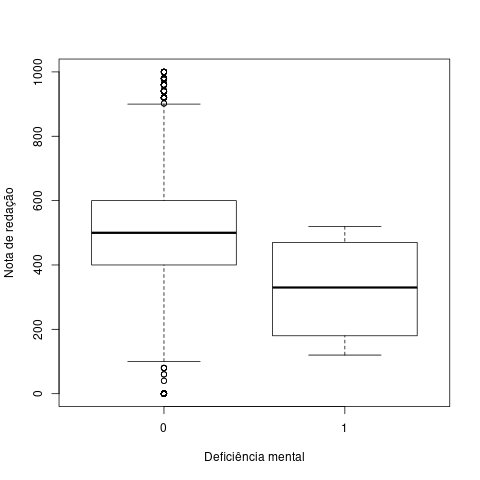
\includegraphics[width=.5\linewidth]{../correlacao_deficiencia_mental.png}
% \caption{Distribuição das notas de redação para candidatos com e sem deficiência mental.}
% \label{fig:correlacao-deficiencia-mental}
% \end{figure}

% \subsubsection{Deficiência física}
% A \reffig{correlacao-deficiencia-fisica} indica que a nota mediana de redação dos candidatos com deficiência física é aproximadamente igual à nota mediana de redação dos candidatos sem deficiência física (em torno de 500).
% No entanto, a proporção de candidatos com nota acima de 500 é menor para portadores de deficiência física.
% \begin{figure}[H]
% \centering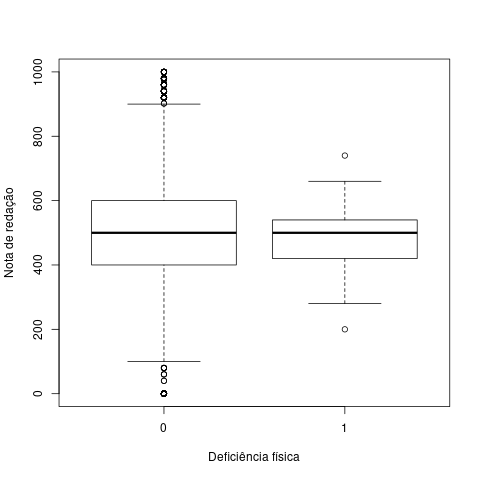
\includegraphics[width=.5\linewidth]{../correlacao_deficiencia_fisica.png}
% \caption{Distribuição das notas de redação para candidatos com e sem deficiência física.}
% \label{fig:correlacao-deficiencia-fisica}
% \end{figure}

\section{Pré-processamento}
\label{sec:pre-processamento}
Nesta etapa, preparamos a base de dados para utilização no algoritmo de classificação.
Optamos por remover colunas majoritariamente por razões técnicas (número de identificação do candidato, por exemplo, além de outros campos descritos a seguir). Consequentemente, colunas que simplesmente suspeitávamos serem poucos relevantes para a classificação, devido à análise estatística previamente realizada, foram mantidas.
Essa abordagem permitiu que a análise estatística atuasse como um guia durante o desenvolvimento do algoritmo de classificação, ao invés de determinar completamente os atributos nele utilizados.

De forma geral, atributos numéricos foram mapeados para um subintervalo de [0, 1] de forma a torná-los aproximadamente igualmente relevantes para a classificação, pelo menos a princípio.
Caso isso não fosse feito, atributos associados a intervalos de valores mais amplos (particularmente as notas nas provas objetivas) execeriam maior influência que os demais.
Similarmente, atributos qualitativos nominais com $C > 2$ categorias foram separados em $C$ atributos booleanos.
Isso foi feito porque a atribuição arbitrária de valores numéricos a cada uma das categorias induziria uma ordenação indevida entre essas categorias.
As operações realizadas durante a normalização são descritas mais detalhadamente a seguir.

\begin{itemize}
    \item Foi criada a coluna UF\_INSC\_IGUAL\_PROVA, que guarda ``1'' se UF\_INSC for igual ao UF\_MUNICIPIO\_PROVA, indicando que o candidato não mudou de estado para fazer a prova. ``0'' caso contrário.
    \item UF\_INSC foi expandido para um total de 26 colunas, cada uma contendo ``1'' ou ``0'' para indicar se o candidato fez a prova nesse estado ou não. Nenhum candidato poder ter mais de um estado marcado como ``1''. Informações adicionais sobre a localização do candidato (nome do município, código do municício, etc.) foram removidas.
    \item De forma similar, TP\_SEXO foi expandido para duas colunas: GENERO\_HOMEM e GENERO\_MULHER, com apenas uma delas sendo marcada como ``1''.
    \item As colunas NOTA\_CN, NOTA\_CH, NOTA\_LC e NOTA\_MT passaram a guardar a nota do candidato em cada uma das provas. Para que o valor fosse consistente de 0 a 1, essa nota foi dividida por 1000.
    \item Várias colunas que guardavam as opções marcadas pelo candidato, gabarito, identificação da prova e afins foram removidas por serem irrelevantes para obtenção do resultado.
    \item A coluna TP\_ESCOLA foi expandida para duas colunas: ESCOLA\_PUBLICA e ESCOLA\_PRIVADA. Para a maioria dos candidatos, o tipo de escola não foi informado, e portanto ambas as colunas ficaram com valor falso. Demais informações sobre a escola e a entidade certificadora do candidato (nome, município, etc.) foram removidas.
    Analogamente, a coluna  ID\_LOCALIZACAO foi expandida para duas colunas: LOCALIZACAO\_URBANA e LOCALIZACAO\_RURAL. Para a maioria dos candidatos, o tipo de localização não foi informado, e portanto ambas as colunas ficaram com valor falso.
    \item A idade foi normalizada para valores de 0 a 1 através de uma divisão por 100. Dessa forma, a menor idade passou a ser 0.12 e a maior idade passou a ser 0.70.
    \item TP\_COR\_RACA foi dividido em 5 colunas, uma com cada cor/raça. Cada uma possui ``1'' se ela é verdadeira para o candidato. Nenhum candidato tem duas dessas colunas como verdadeiras.
    \item Analogamente, TP\_ESTADO\_CIVIL foi dividido em 4 colunas booleanas: ESTADO\_CIVIL\_SOLTEIRO, ESTADO\_CIVIL\_CASADO, ESTADO\_CIVIL\_DIVORCIADO e ESTADO\_CIVIL\_VIUVO.
    \item ST\_CONCLUSAO foi dividido em 4 colunas seguindo o mesmo princípio: ENSINO\_MEDIO\_CONCLUIDO (alunos que já haviam concluído o Ensino Médio quando a prova foi aplicada), ENSINO\_MEDIO\_EM\_2012 (alunos que estavam concluindo o Ensimo Médio no mesmo ano de aplicação da prova), ENSINO\_MEDIO\_DEPOIS\_2012 (alunos que só concluiríam o Ensino Médio em anos posteriores à aplicação da prova) e ENSINO\_MEDIO\_NAO\_FAZ (alunos que nem haviam concluído previamente nem estavam cursando o Ensino Médio). O ano exato de conclusão do Ensino Médio, quando informado, foi descartado.
\end{itemize}

\section{Classificação}
\label{sec:classificacao}
O objetivo final do trabalho foi a classificação dos candidatos em quatro classes, de acordo com a nota obtida na prova de redação: ``ruim'', ``regular'', ``boa'' e ``ótima''.
A determinação da classe de cada candidato foi feita através da divisão do dataset original em quartis: candidatos no primeiro quartil foram classificados como ótimos, candidatos no segundo quartil como bons, e assim por diante.
Esse processo resulta em uma divisão equitativa dos candidatos em classes, e consequentemente simplifica uma avaliação justa do algoritmo de classificação desenvolvido.

O algoritmo de classificação utilizado foi o \emph{k-Nearest Neighbors} (\emph{k-NN}).
Durante o treinamento desse algoritmo, todas as observações do conjunto de treinamento são convertidas em vetores no espaço de características.
(Por isso, é importante que a etapa de pré-processamento gere apenas atributos numéricos.)
Depois disso, sempre que uma nova observação precisa ser classificada, são identificadas as $k$ observações mais próximas dela no conjunto de treinamento (no nosso caso, de acordo com a distância de Euclides).
A classe predita é simplesmente a classe mais frequente dentre essas $k$ observações.
Em todos os experimentos realizados, utilizamos $\nicefrac{2}{3}$ da base para treinamento e o restante para avaliação do algoritmo.

Amparados na análise estatística previamente realizada, elegemos um conjunto inicial de atributos que julgamos relevantes para a classificação: IDADE, IN\_DEFICIENCIA\_MENTAL, NOTA\_CN, NOTA\_CH, NOTA\_LC, NOTA\_MT, ESCOLA\_PRIVADA e LOCALIZACAO\_RURAL.
Em seguida, refinamos essa seleção inicial através de experimentos envolvendo a inserção e a remoção de atributos, sempre utilizando $k=3$.
O conjunto de atributos que apresentou melhor resultado foi o seguinte: GENERO\_HOMEM, IDADE, IN\_DEFICIENCIA\_MENTAL, NOTA\_CN, NOTA\_CH, NOTA\_LC, NOTA\_MT e ESCOLA\_PRIVADA.
Também experimentamos multiplicar os valores de alguns atributos (em especial, notas nas provas objetivas) por números reais maiores que um, de forma a atribuir-lhes maior peso, mas não houve melhora significativa no resultado.

Finalmente, avaliamos a acurácia do algoritmo desenvolvido com diferentes valores de $k$.
As Fig.~\ref{fig:tab1}--\ref{fig:tab100} mostram, para todos os pares de classes $(X, Y)$, quantos candidatos da classe $X$ foram classificados como sendo da classe $Y$.
As Fig.~\ref{fig:graf1}--\ref{fig:graf100} sumarizam os tipos de erros cometidos pelo algoritmo.
Os gráficos evidenciam que, em geral, melhores resultados são obtidos com maiores valores de $k$.
No entanto, essa melhora ocorre principalmente para as classes mais extremas (''ótimo`` e ''ruim```); os resultados da classe ''regular`` melhoram de forma menos significativa e os resultados da classe ''bom`` pioram.

\begin{figure}[H]
\centering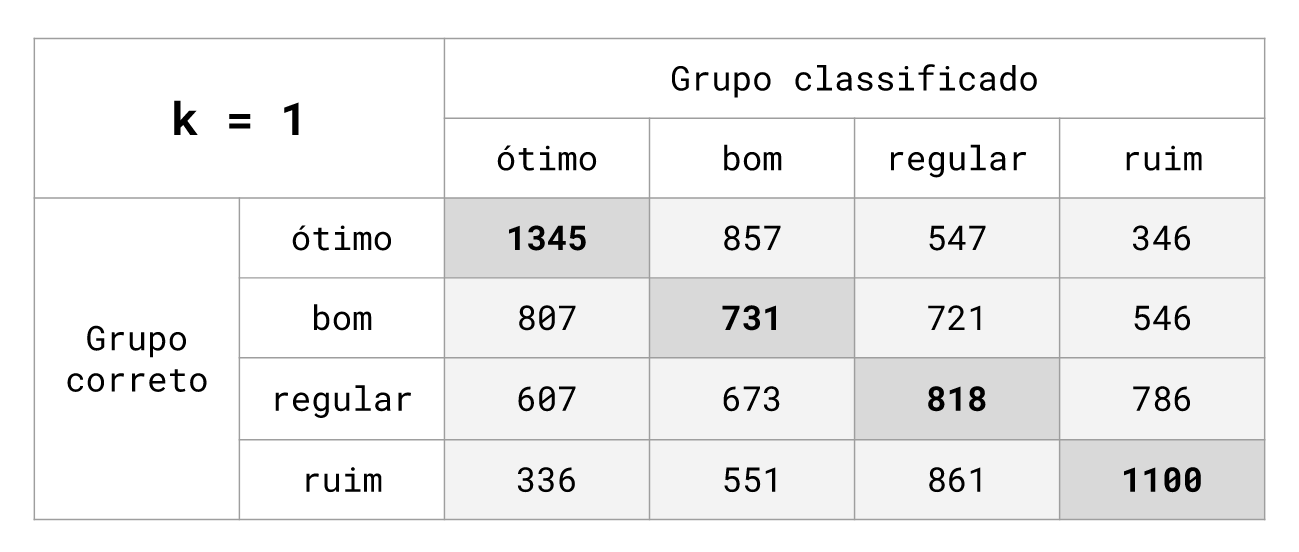
\includegraphics[width=.60\linewidth]{plot-white1.png}
\caption{Análise dos resultados obtidos pelo \emph{k-NN} com k=1.}
\label{fig:tab1}
\end{figure}

\begin{figure}[H]
\centering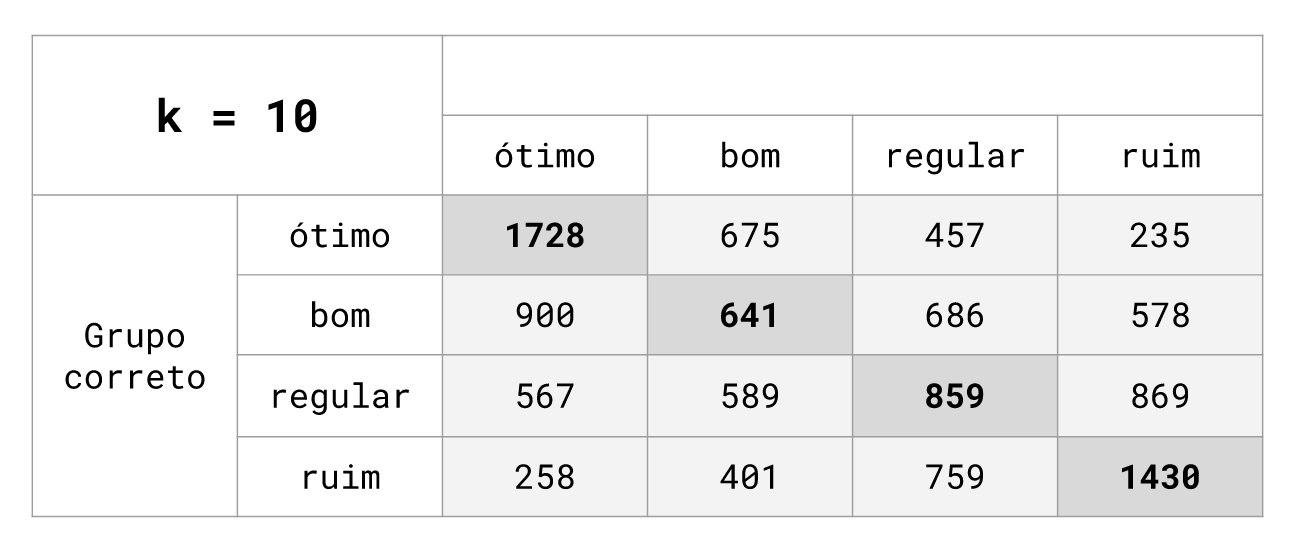
\includegraphics[width=.60\linewidth]{plot-white10.png}
\caption{Análise dos resultados obtidos pelo \emph{k-NN} com k=10.}
\label{fig:tab10}
\end{figure}

\begin{figure}[H]
\centering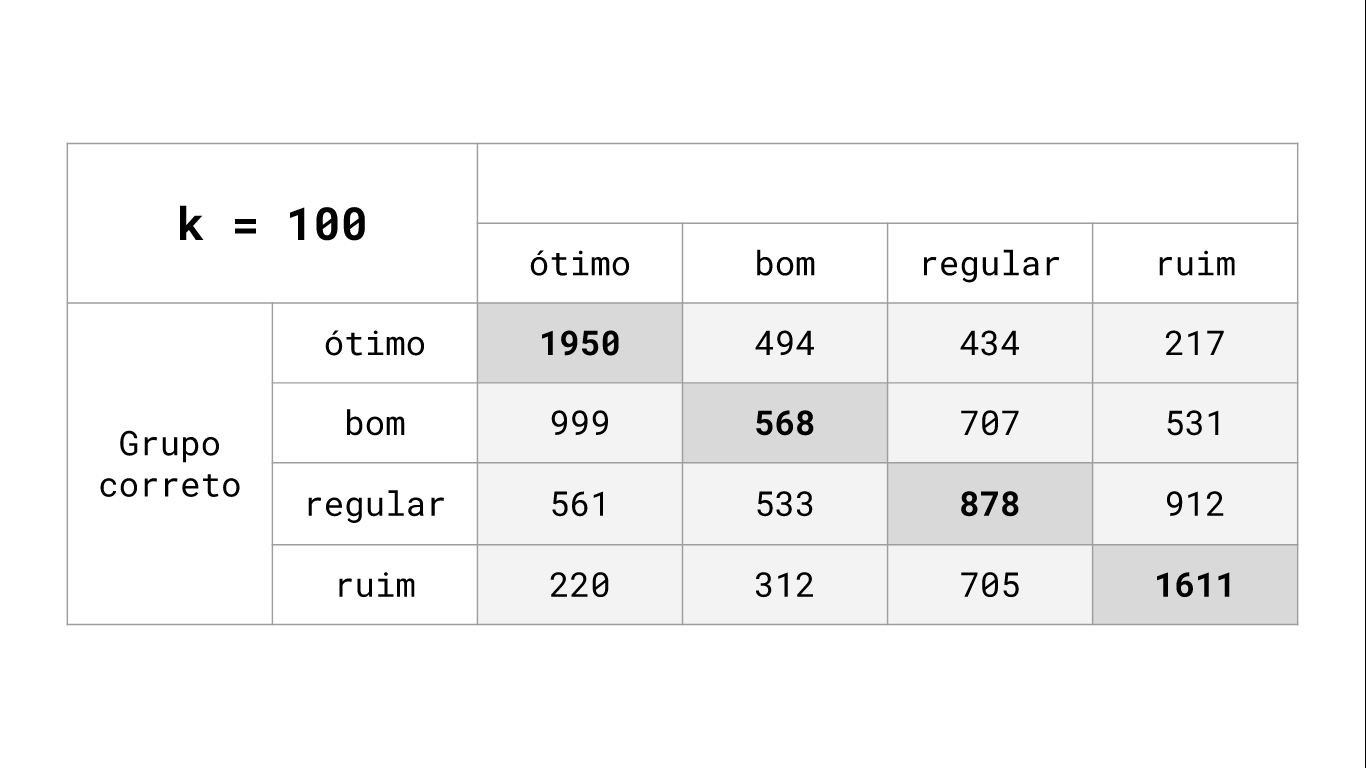
\includegraphics[width=.60\linewidth]{plot-white100.png}
\caption{Análise dos resultados obtidos pelo \emph{k-NN} com k=100.}
\label{fig:tab100}
\end{figure}

\begin{figure}[H]
\centering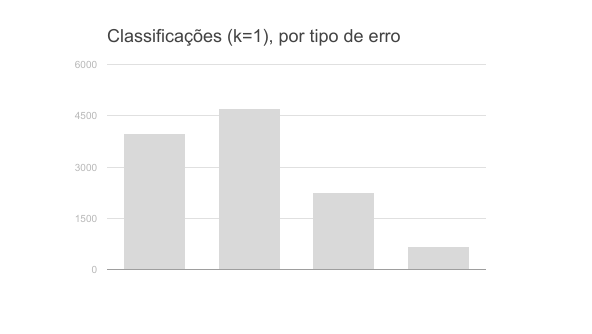
\includegraphics[width=.65\linewidth]{graf-white1.png}
\caption{Classificações por tipo de erro do \emph{k-NN} com k=1.}
\label{fig:graf1}
\end{figure}

\begin{figure}[H]
\centering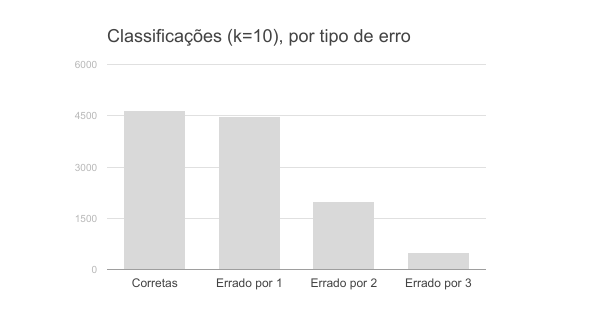
\includegraphics[width=.65\linewidth]{graf-white10.png}
\caption{Classificações por tipo de erro do \emph{k-NN} com k=10.}
\label{fig:graf10}
\end{figure}

\begin{figure}[H]
\centering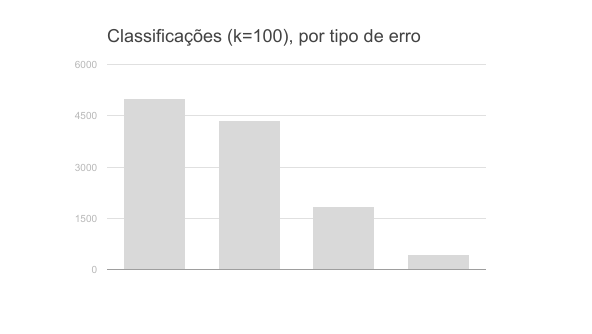
\includegraphics[width=.65\linewidth]{graf-white100.png}
\caption{Classificações por tipo de erro do \emph{k-NN} com k=100.}
\label{fig:graf100}
\end{figure}

\section{Conclusão}
\label{sec:conclusao}
Os experimentos realizados sugerem que os melhores resultados são obtidos pelo \emph{k-NN} com $k=100$

\end{document}
